
\subsection{Transformer Core Measurements}
\label{sec:transformer}

An alternative technique similar to the standard method of magnetic
materials characterization via magnetic induction was also used to
measure changes in $\mu$.  In this measurement technique, the witness
cylinder was used as the core of a transformer.  Two coils (primary
and secondary) were wound on the witness cylinder using multistranded
20-gauge copper wire.  The windings were made as tight as possible,
but not so tight as to potentially stress the material.  The windings
were not potted in place.  Three witness cylinders were tested.  Data
were acquired using different numbers of turns on both the primary and
secondary coils (from 6 to 48 on the primary, and from 7 to 24 on the
secondary).

Fig.~\ref{fig:transformer} shows a picture of one of the witness
cylinders, wound as described.  It also shows a schematic diagram of
the measurement setup, which we now use to describe the measurement
principle.

\begin{figure}[h!]
  \begin{center}
    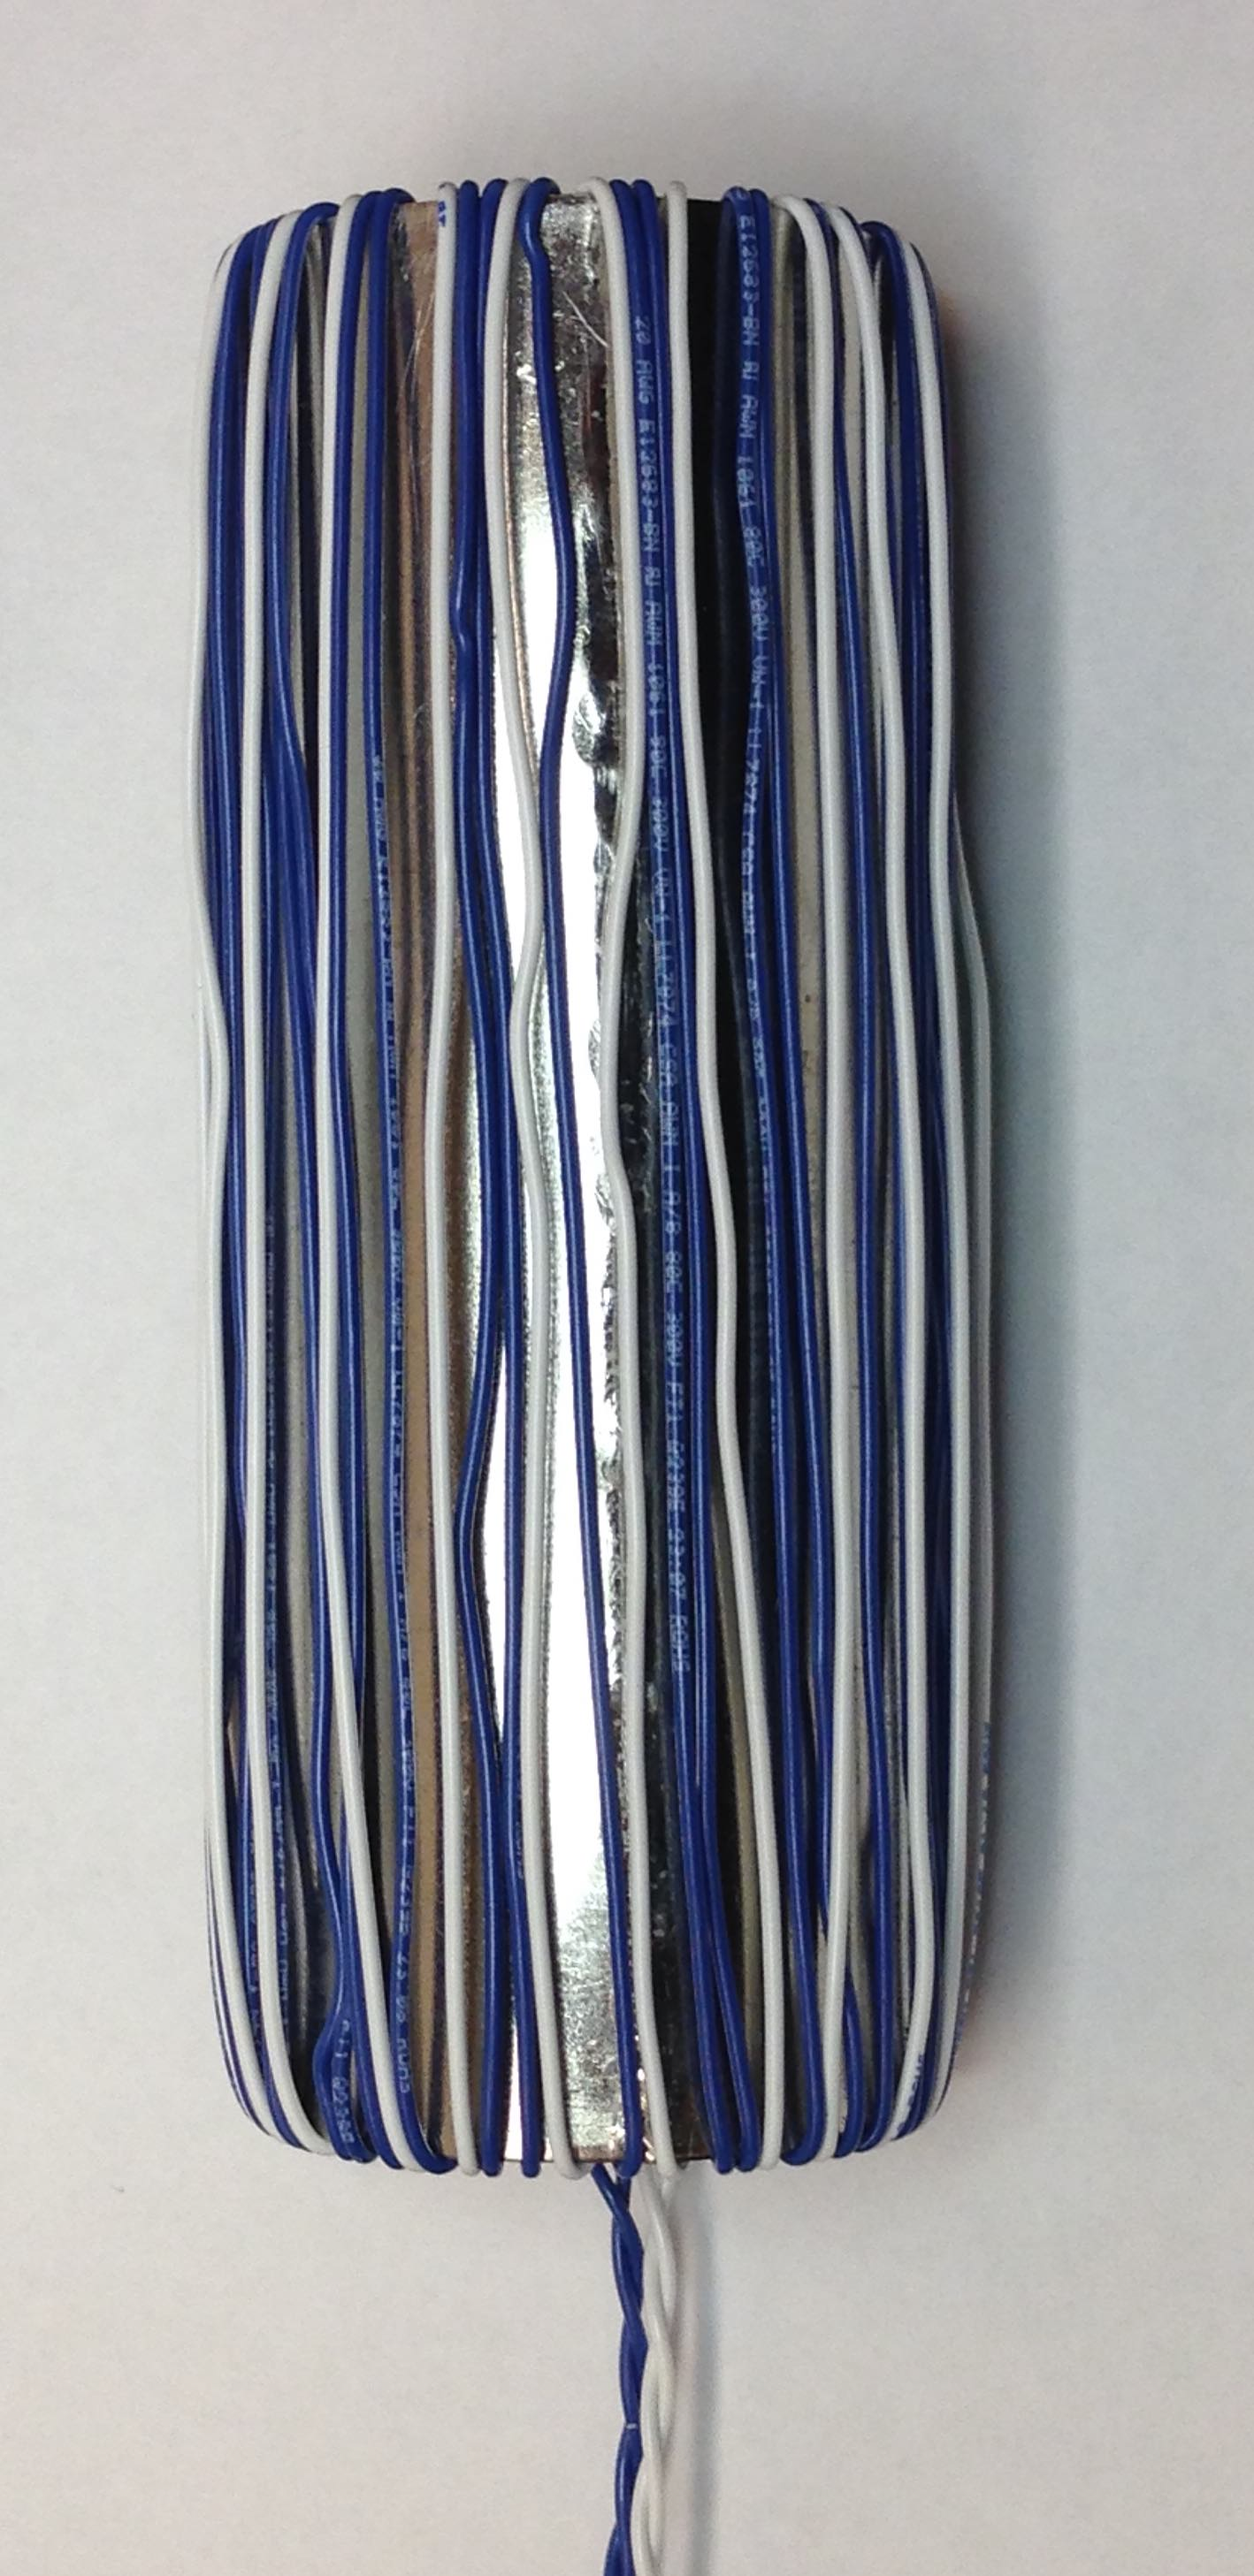
\includegraphics[height=3cm]{picture.png}\hskip1cm
    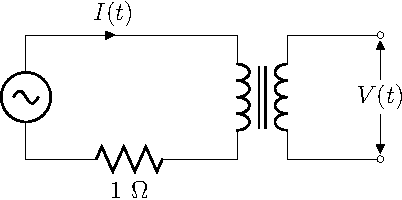
\includegraphics[height=3cm]{figure4-crop.pdf}
    \caption{Photograph of a witness cylinder showing transformer
      windings (left) and schematic of the transformer measurement
      (right).  The primary coil was driven by the sine-out of an
      SR830 lock-in amplifier, which was also used to demodulate
      induced voltage $V(t)$ in the secondary coil. The driving
      current $I(t)$ was sensed by measuring the voltage across a
      stable 1~$\Omega$ resistor.}
    \label{fig:transformer}
  \end{center}
\end{figure}


% Table 9 on page 65 of Taraneh's report shows the different windings.
% Can guess which core is which.

%In the end, a transformer with 48 windings on the primary and 21
%windings on the secondary was used.

%This enabled more saturation of the material.

The primary coil generated an AC magnetic field as a function of time
$H(t)$, while the secondary coil was used to measure the emf induced
by the time-varying magnetic flux proportional to $dB(t)/dt$.  To a
good approximation
\begin{equation}
H_m(t)=\frac{N_pI(t)}{2\pi R}
\end{equation}
where $N_p$ is the number of turns in the primary, $I(t)$ is the
current in the primary, and $R$ is the radius of the witness cylinder,
and
\begin{equation}
\frac{dB_m(t)}{dt}=\dot{B}_m(t)=\frac{V(t)}{b\ell}
\label{eqn:bdot}
\end{equation}
where $V(t)$ is the voltage generated in the secondary, and $b$ and
$\ell$ are the thickness and length of the witness cylinder
respectively.  For a sinusoidal drive current $I(t)$, and under the
assumption that $B_m(t)=\mu H_m(t)$ with $\mu$ being a constant, the
voltage generated in the secondary $V(t)$ should be sinusoidal and out
of phase with the primary current.

The internal oscillator of an SR830 lock-in amplifier was used to
generate $I(t)$.  This was monitored by measuring the voltage across a
1~$\Omega$ resistor with small temperature coefficient in the primary
loop. The lock-in amplifier was then used to demodulate $V(t)$ into
its in-phase $V_X$ and out-of-phase $V_Y$ components (or equivalently
$\dot{B}_m(t)$ being demodulated into $\dot{B}_{m,X}$ and
$\dot{B}_{m,Y}$, as in equation~(\ref{eqn:bdot})).  The experiment was
done at 1~Hz with $H_m(t)$ as small as possible, typically 0.1~A/m in
amplitude, to measure the slope of the minor $B_m-H_m$ loops near the
origin of the $B_m-H_m$ space.

The temperature of the core was measured continuously using the same
thermocouple arrangement described previously. Measurements of $V_Y$
as a function of temperature would then signify a change in $\mu$ with
temperature.  In general, we used ambient temperature variations for
the measurements, similar to the procedure used for our axial
shielding factor measurements.

% Although we would have preferred to measure at even lower frequencies
% and amplitudes, these settings were found to be the minimum possible
% before noise would make it impossible to measurement the long-term
% (hours) evolution of the $X$ and $Y$ readings.

The naive expectation is that the out-of-phase $V_Y$ component should
signify a non-zero $\mu$, and the in-phase $V_X$ component should be
zero.  In practice, due to a combination of saturation, hysteresis,
eddy-current losses, and skin-depth effects, the $V_X$ component is
nonzero.  It was found experimentally that keeping the amplitude of
$H_m(t)$ small compared to the apparent coercivity ($\sim 3$~A/m for
the 0.16~cm thick material at 1~Hz frequencies) ensured that the $V_Y$
component was larger than the $V_X$ component.  This is displayed
graphically in Fig.~\ref{fig:data_and_simulation}, where the
dependence of $\dot{B}_{m,Y}$ and $\dot{B}_{m,X}$ on the amplitude of
the applied $H_m(t)$ is displayed, for a driving frequency of 1~Hz.
Clearly the value of $\dot{B}_{m,X}$ can be considerable compared to
$\dot{B}_{m,Y}$, for larger $H_m$ amplitudes near the coercivity.  At
larger amplitudes, the material goes into saturation.  Both
$\dot{B}_{m,Y}$ and $\dot{B}_{m,X}$ eventually decrease as expected at
amplitudes much greater than the coercivity.

To understand the behavior in Fig.~\ref{fig:data_and_simulation}, a
theoretical model of the hysteresis based on the work of
Jiles~\cite{jiles1994frequency} was used.  The model contains a number of
adjustable parameters.  We adjusted the parameters based on our
measurements of $B_m-H_m$ loops including the initial magnetization
curve.  These measurements were performed separately from our lock-in
amplifier measurements, using an arbitrary function generator and a
digital oscilloscope to acquire them.  The measurements were done at
frequencies from 0.01 to 10~Hz.  It was found that the frequency
dependence predicted by Ref.~\cite{jiles1994frequency} gave relatively good
agreement with the measured $B_m-H_m$ loops once the five original
(Jiles-Atherton~\cite{jiles1984theory,jiles1986theory}) parameters were tuned.

For the parameters of the (static) Jiles-Atherton model, we used
$B_s=0.45$~T, $a=3.75$~A/m, $k=2.4$~A/m, $\alpha=2\times 10^{-6}$,
$c=0.05$, which were tuned to our $B_m-H_m$ curve measurements.  For
classical losses, we used the parameters $\rho=5.7\times
10^{-7}~\Omega\cdot$m, $d=1.6$~mm (the thickness of the material), and
$\beta=6$ (geometry factor).  These parameters were not tuned, but
taken from data.  For anomalous losses we used the parameters
$w=0.005$~m and $H_0=0.0075$~A/m, which we also did not tune, instead
relying on the tuning performed in Ref.~\cite{jiles1994frequency}.

These parameters were then used to model the measurement presented in
Fig.~\ref{fig:data_and_simulation}, including the lock-in amplifier
function.  As shown in Fig.~\ref{fig:data_and_simulation}, trends in
the measurements and simulations are fairly consistent.  The sign of
$\dot{B}_{m,X}$ relative to $\dot{B}_{m,Y}$ is also correctly
predicted by the model (we have adjusted them both to be positive, for
graphing purposes).  We expect that with further tuning of the model,
even better agreement could be achieved.

\begin{figure}[h!]
  \begin{center}
    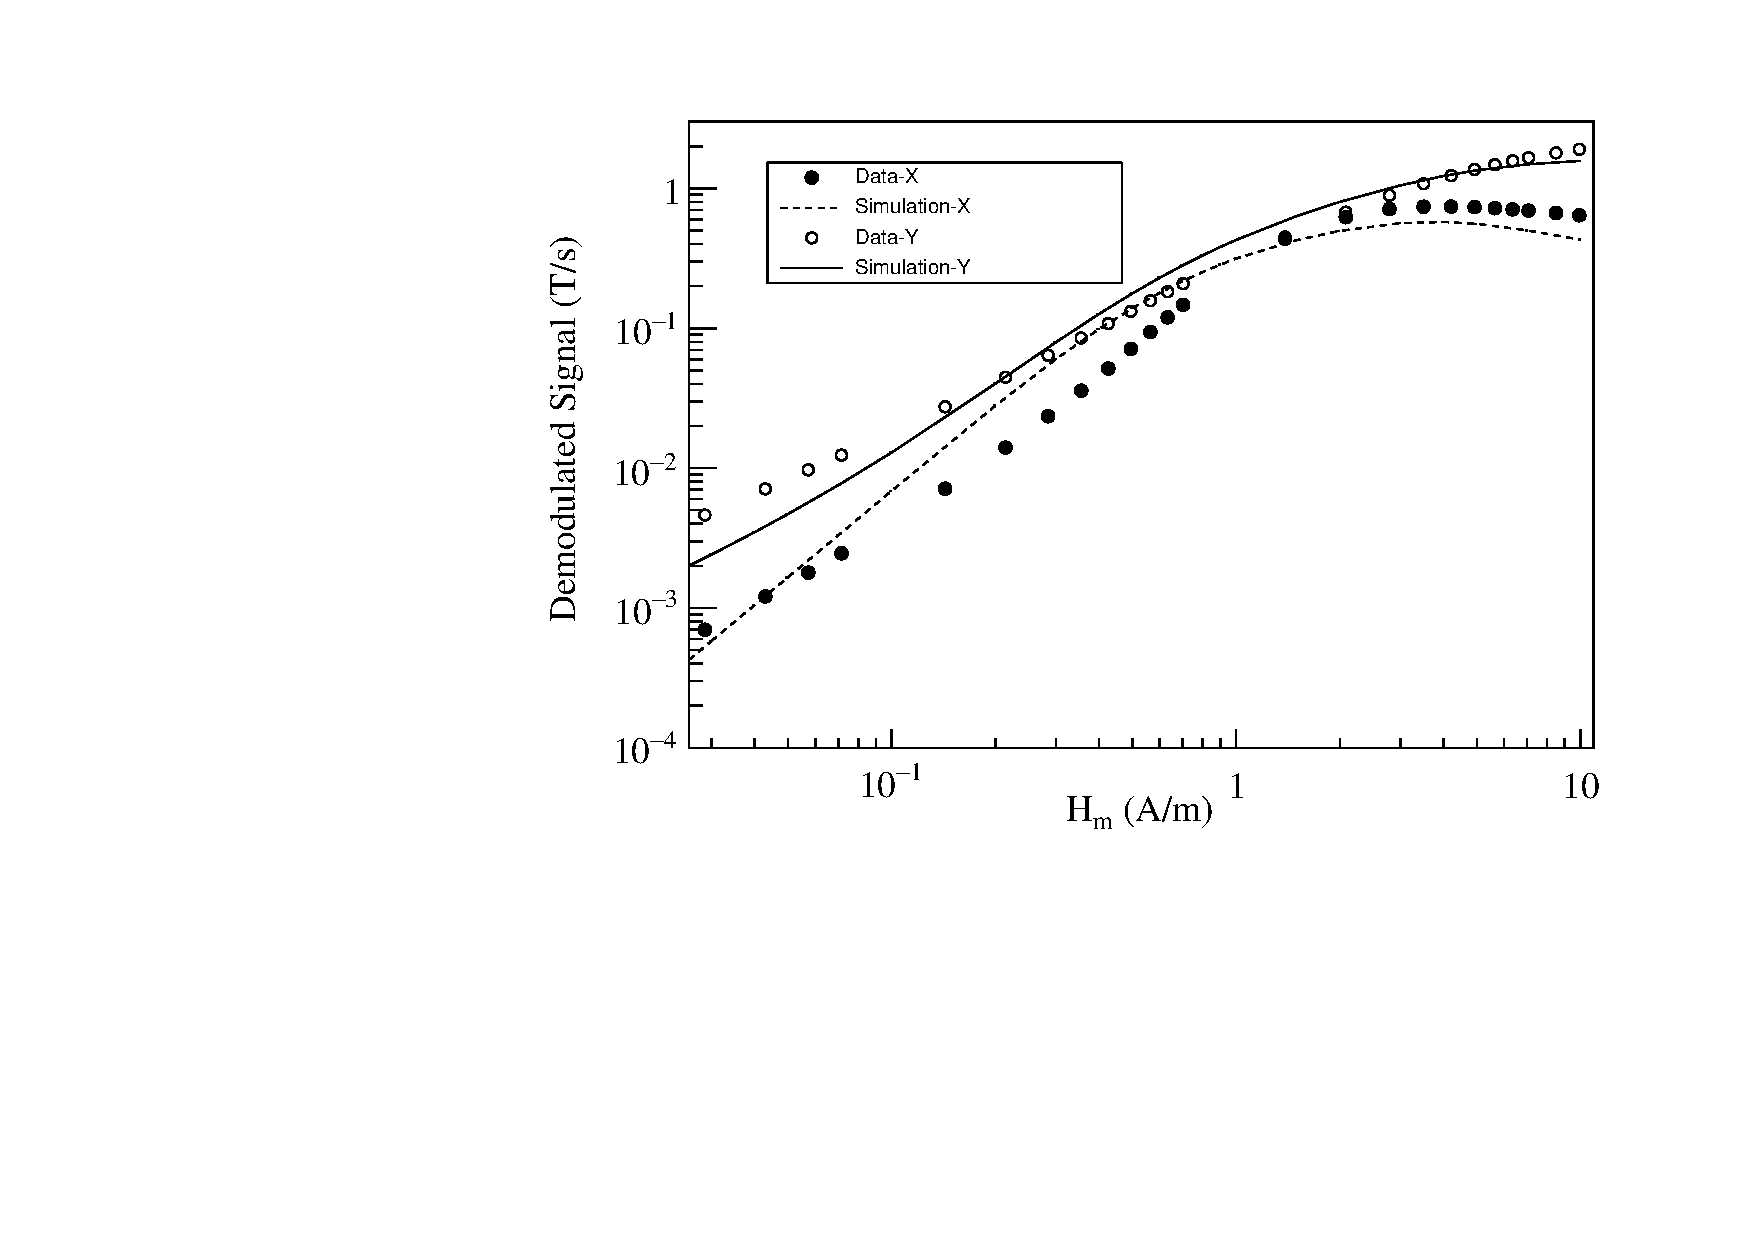
\includegraphics[width=\textwidth]{Jiles_and_data.pdf}
    \caption{$\dot{B}_{m,X}$ and $\dot{B}_{m,Y}$ as a function of
      amplitude of the applied $H_m$ field at 1~Hz.  Points show the
      acquired data.  Curves display the simulation based on the model
      described in the text.}
    \label{fig:data_and_simulation}
  \end{center}
\end{figure} 

The model of Ref.~\cite{jiles1994frequency} makes no prediction of the
temperature dependence of the parameters.  Ideally, the temperature
dependence of $\dot{B}_{m,Y}$ and $\dot{B}_{m,X}$ under various
conditions could be used to map out the temperature dependence of the
parameters.  However, this is beyond the scope of the present work.

We make the simplifying assumption that temperature dependence of
$\dot{B}_{m,Y}$ may be approximately interpreted as the temperature
dependence of a single parameter $\mu$, i.e. that
\begin{equation}
\frac{1}{\dot{B}_{m,Y}}\frac{d\dot{B}_{m,Y}}{dT}=\frac{1}{\mu}\frac{d\mu}{dT}.
\end{equation}
This is justified in part by our selection of measurement parameters
(the amplitude of $H_m=0.1$~A/m and a measurement frequency of 1~Hz)
which ensure that $\dot{B}_{m,Y}$ dominates over $\dot{B}_{m,X}$.

We assign no additional systematic error for this simplification, and
all our results are subject to this caveat.  We comment further that
in our measurements of the axial shielding factor (presented in
Section~\ref{sec:axial}), the same caveat exists.  In that case the
in-phase component dominates the demodulated fluxgate signal.  In a
sense, measuring $\mu(T)$ itself is always an approximation, because
it is actually the parameters of minor loops in a hysteresis curve
which are measured.  In reality, our results may be interpreted as a
measure of the temperature-dependence of the slopes of minor loops
driven by the stated $H_m$.

Measurements of $\frac{1}{\dot{B}_{m,Y}}\frac{d\dot{B}_{m,Y}}{dT}$ as
a function of $T$ were made.  In general, the data mimicked the
behavior of the axial shielding factor measurements, giving a similar
level of linearity with temperature as the data displayed in
Fig.~\ref{fig:B_vs_Temp}.  Other similar behaviors to those
measurements were also observed, for example: (a) when the temperature
slope changed sign, $\dot{B}_{m,Y}$ would temporarily give a different
slope with temperature, (b) the measured value of
$\frac{1}{\dot{B}_{m,Y}}\frac{d\dot{B}_{m,Y}}{dT}$ depended on a
variety of factors, most notably a dependence on which of the three
witness cylinders was used for the measurement, and on differences
between subsequent measurements using the same cylinder.

\begin{table}
\begin{center}
\begin{tabular}{cccc}\hline
Trial & $\frac{1}{\dot{B}_{m,Y}}\frac{d\dot{B}_{m,Y}}{dT}$ & core \\
\#    & (\%/K) & used \\\hline
 1 & 0.15 & $\alpha$ \\
 2 & 0.03 & $\alpha$ \\
 3 & 0.04 & $\alpha$ \\
 4 & 0.06 & $\alpha$ \\
 5 & 1.07 & $\beta$  \\
 6 & 0.93 & $\beta$  \\
 7 & 0.88 & $\beta$  \\
 8 & 0.88 & $\beta$  \\
 9 & 0.09 & $\alpha$ \\
10 & 1.23 & $\beta$  \\
11 & 2.15 & $\beta$  \\
12 & 1.85 & $\beta$  \\
13 & 1.20 & $\beta$  \\
14 & 0.77 & $\gamma$ \\\hline
\end{tabular}
\caption{Summary of data acquired for the transformer core
  measurements.  Three different witness cylinders, arbitrarily
  labeled $\alpha$, $\beta$, and $\gamma$, were used for the
  measurements.  A 1~Hz excitation frequency was used with amplitudes
  for $H_m$ ranging from 0.1 to 0.3~A/m.  Fluctuations in the
  temperature ranged from 21-24$^\circ$C and measurement times over a
  10-80 hour period are included.  Other data acquired for systematic
  studies are not included in the table.\label{tab:transformer}}
\end{center}
\end{table}



Table~\ref{tab:transformer} summarizes our measurements of the
relative slope $\frac{1}{\dot{B}_{m,Y}}\frac{d\dot{B}_{m,Y}}{dT}$ for
a variety of trials, witness cylinders, and numbers of windings.  The
data show a full range of $0.03-2.15$\%/K for
$\frac{1}{\mu}\frac{d\mu}{dT}=\frac{1}{\dot{B}_{m,Y}}\frac{d\dot{B}_{m,Y}}{dT}$,
again naively assuming the material to be linear as discussed above.
The sign of the slope of $\mu(T)$ was the same as the axial shielding
factor technique.

A dominant source of variation between results in this method arose
from properties inherent to each witness cylinder.  One of the
cylinders (referred to as $\beta$ in Table~\ref{tab:transformer}) gave
temperature slopes consistently larger
$\frac{1}{\mu}\frac{d\mu}{dT}\sim 0.88-2.15$\%/K than the other two
$\frac{1}{\mu}\frac{d\mu}{dT}\sim 0.03-0.77$\%/K (referred to as
$\alpha$ and $\gamma$, with some evidence that $\gamma$ had a larger
slope than $\alpha$).  We expect this indicates some difference in the
annealing process or subsequent treatment of the cylinders, although
to our knowledge the treatment was controlled the same as for all
three cylinders.  Since our goal is to provide input to future EDM
experiments on the likely scale of the temperature dependence of $\mu$
that they can expect, we phrase our result as a range covering all
these results.

Detailed measurements of the effect of degaussing were conducted for
this geometry.  The ability to degauss led us ultimately to select a
larger number of primary turns (48) so that we could fully saturate
the core using only the lock-in amplifier reference output as a
current source.  A computer program was used to control the lock-in
amplifier in order to implement degaussing.  A sine wave with the
measurement frequency (typically 1~Hz) was applied at the maximum
lock-in output power.  Over the course of several thousand
oscillations, the amplitude was decreased linearly to the measurement
amplitude ($\sim 0.1$~A/m).  After degaussing with parameters
consistent with the recommendations of
Refs.~\cite{thiel2007demagnetization,altarev2015minimizing}, the measured temperature
slopes were consistent with our previous measurements where no
degaussing was done.

Other systematic errors found to contribute at the $<0.1\%$/K level
were: motion of the primary and secondary windings, stability of the
lock-in amplifier and its current source, and stability of background
noise sources.

To summarize, the dominant systematic effects arose due to different
similarly prepared cores giving different results, and due to
variations in the measured slopes in multiple measurements on the same
core.  The second of these is essentially the same error encountered
in our axial shielding factor measurements.  We expect it has the same
source; it is possibly a property of the material, or an additional
unknown systematic uncertainty.
